Der Compton-Effekt beschreibt die Streuung eines Photons an einem quasi-freien Elektron. Dabei ist
die Photonenergie $E_\gamma$ groß im Vergleich zur Bindungsenergie $E_{\text{Bindung}}$ der
Hüllenelektronen, sodass diese vernachlässigt werden kann.

\[ \gamma + \text{Atom} \longrightarrow \gamma + e^- +\text{Ion}\]

Das Photon wird von seiner usprünglichen Bahn abgelenkt und seine Wellenlänge durch den
Energieübertrag auf das Elektron geändert. 

\begin{figure}[H]
	\centering
	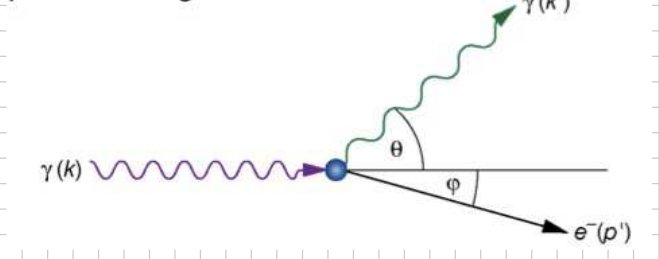
\includegraphics[width=0.75\textwidth]{6-kinematik.jpg}
	\caption{Kinematik des Compton-Effekts	}
	\label{}
\end{figure}

Die Energie des gestreuten Photons lässt sich aus der Kinematik als Funktion des Streuwinkels
berechnen:

\[ E_\gamma' = \frac{E_\gamma}{1+ \frac{E_\gamma}{m_ec^2}\left(1-\text{cos}\,\Theta\right)} \]

Aus der QED und Berechnung der Feynmangraphen erhalten wir die Klein-Nishina-Formel für den
winkelabhängigen Streuquerschnitt eines Photons an einem Elektron (s. Abb. \ref{fgraph2}):

\[ \frac{\mathrm{d}\sigma}{\mathrm{d}\Omega} = \frac{r_e^2}{2
\left[1+\epsilon\left(1-\text{cos}\,\Theta \right) \right]^2} \left(1+\text{cos}^2\,\Theta +
\frac{\epsilon^2\left(1-\text{cos}\,\Theta \right)^2}{1+\epsilon\left(1- \text{cos}\,\Theta \right)}
\right)
\]

mit $\epsilon = \frac{E_\gamma}{m_ec^2}$.

\begin{figure}[H]
	\begin{minipage}[b]{0.5\textwidth}
		\begin{figure}[H]
		\centering
		\includesvg[svgpath=bilder/1-1/]{feynman3}
		\end{figure}
	\end{minipage}
	\hspace{5mm} 
	\begin{minipage}[b]{0.5\textwidth}
		\begin{figure}[H]
		\centering
		\includesvg[svgpath=bilder/1-1/]{feynman4}
		\vspace{3mm}
		\end{figure} 
	\end{minipage} 
\end{figure}


\begin{figure}[H]
	\centering
	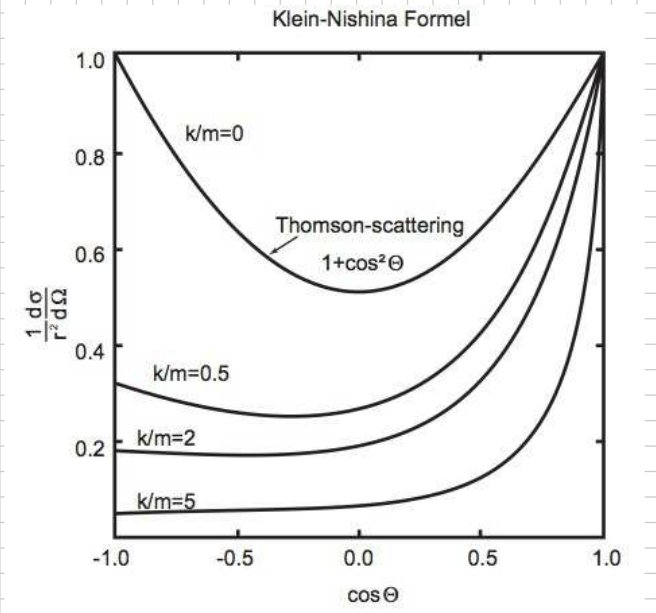
\includegraphics[width=0.5\textwidth]{8-kleinNishinaFormel.jpg}
	\caption{Winkelverteilung für Compton-Streuung}
	\label{kleinnishina}
\end{figure}

In Abb. \ref{kleinnishina} ist die Winkelverteilung für die Compton-Streuug zu sehen. Für großes
$E_\gamma$ ergibt sich ein starker Anstieg in Vorwärtsrichtung.
\\
Nach Integration über den Raumwinkel und Summation über alle Elektronen eines Atoms erhält man den
totalen Compton-Wirkungsquerschnitt pro Atom:

\[\sigma_{\text{Compton}} = 2\pi \cdot r_e^2\cdot Z \cdot
\left[\frac{1+\epsilon}{\epsilon}\left( \frac{2(1+\epsilon)}{1+2\epsilon} -
\frac{1}{\epsilon}\,\text{ln}(1+2\epsilon) \right) + \frac{1}{2\epsilon}\,\text{ln}(1+2\epsilon) -
\frac{1+3\epsilon}{(1+2\epsilon)^2} \right] \]

\[\Rightarrow\,\, \sigma_{\text{Compton}} \sim N(e^-) \sim Z  \]

\begin{figure}[H]
	\centering
	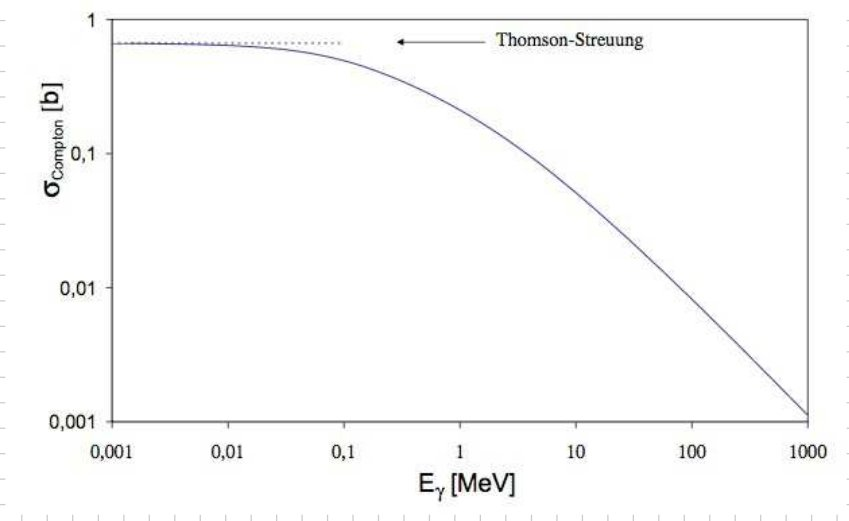
\includegraphics[width=0.75\textwidth]{9-thomsonStreuung.jpg}
	\caption{Compton-Wirkungsquerschnitt}
	\label{comptonwq}
\end{figure}

Im Detektor wird häufig nur die Energie $E_{\text{kin}}$ des Rückstoßelektrons nachgewiesen,

\[T= E_\gamma -E_\gamma'.  \]

Der Wirkungsquerschnitt hierfür ist

\[\frac{\mathrm{d}\sigma}{\mathrm{d}T} = \frac{\pi\cdot r_e^2}{m_e\cdot c^2\cdot \epsilon^2} \left[
2+ \frac{t^2}{\epsilon^2(1-t)^2} +\frac{t}{1-t}\left(t-\frac{2}{\epsilon} \right) \right] \]

mit $t=\frac{T}{E_\gamma}$.
\\
Die maximalen Elekronenenergie für ein rückwärts-gestreutes Photon (d.h. $\text{cos}\,\Theta=-1$)
ist

\[T_{\text{max}} = E_\gamma\cdot \frac{2\epsilon}{1+2\epsilon}. \] 

Dies wird auch als Compton-Kante bezeichnet und liegt im Energiespektrum des Detektors etwas
unterhalb des Photopeaks.

\begin{figure}[H]
	\centering
	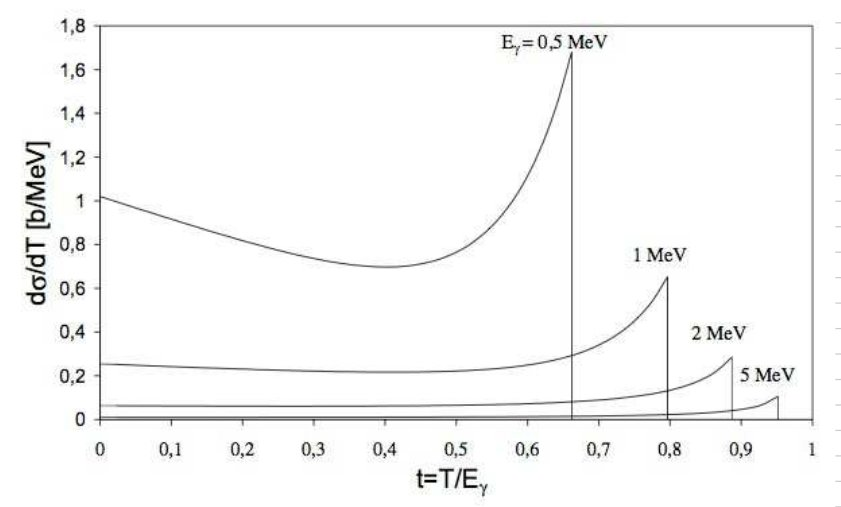
\includegraphics[width=0.75\textwidth]{10-comptonKante.jpg}
	\caption{Compton-Querschnitte der normierten kinetischen Energie}
	\label{comptonTmax}
\end{figure}

Mit wachsendem $E$ gilt:

\[E_\gamma'(\Theta=\pi) \approx \frac{m_ec^2}{2}~~~~~\text{für}~~E_\gamma>>m_ec^2  \]

d.h. die Energie des gestreuten Photons entspricht der Hälfte der Elektronmasse.